%                      Code_Saturne version 1.3
%                      ------------------------
%
%     This file is part of the Code_Saturne Kernel, element of the
%     Code_Saturne CFD tool.
% 
%     Copyright (C) 1998-2007 EDF S.A., France
%
%     contact: saturne-support@edf.fr
% 
%     The Code_Saturne Kernel is free software; you can redistribute it
%     and/or modify it under the terms of the GNU General Public License
%     as published by the Free Software Foundation; either version 2 of
%     the License, or (at your option) any later version.
% 
%     The Code_Saturne Kernel is distributed in the hope that it will be
%     useful, but WITHOUT ANY WARRANTY; without even the implied warranty
%     of MERCHANTABILITY or FITNESS FOR A PARTICULAR PURPOSE.  See the
%     GNU General Public License for more details.
% 
%     You should have received a copy of the GNU General Public License
%     along with the Code_Saturne Kernel; if not, write to the
%     Free Software Foundation, Inc.,
%     51 Franklin St, Fifth Floor,
%     Boston, MA  02110-1301  USA
%
%-----------------------------------------------------------------------
\section{General description}
%----------------

	\subsection{Objective}
%-----------------------------

This aim of this case is to tackle the merging of initially separate meshes into
a single fluid domain. The questions of mesh pasting and hanging nodes will be
addressed. The test case will then be used to present more complex calculations,
with time dependent variables and Fortran user routines.


	\subsection{Description of the configuration}
%-----------------------------------------------

The fluid domain is composed of three separate meshes, very roughly representing
elements of a nuclear pressurized water reactor vessel: 
\begin{itemize}
	\item the downcomer
	\item the vessel's bottom
	\item the lower core plate and core 
\end{itemize}

Figure \ref{figante21} represents the complete domain. The flow circulates from
the top left horizontal junction to the right vertical outlet. 

\begin{figure}[h!]
\begin{center}
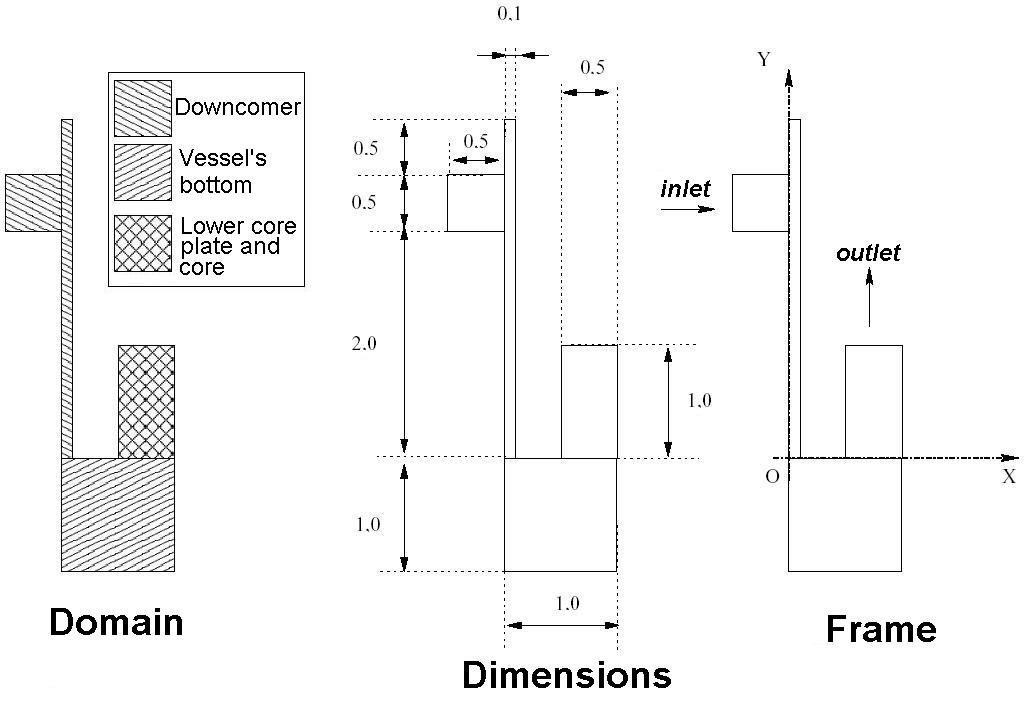
\includegraphics[width=9cm,height=6cm]{\repgraphics/fig04.jpg} 
\caption{Geometry of the complete domain}
\label{figante21}
\end{center}
\end{figure}


	\subsection{Characteristics}
%----------------------------------

The characteristics of the geometry and the flow are:
\begin{center}
\begin{tabular}{|l|c|}
\hline
Height of downcomer & $H = 3.00\ m$ \\
\hline 
Thickness of downcomer & $E_{d} = 0.10\ m$ \\ 
\hline 
Diameter of the inlet cold branch & $D_{b} = 0.50\ m$ \\ 
\hline 
Height of vessel's bottom & $H_{fc} = 1.00\ m$ \\ 
\hline 
Width of vessel's bottom & $l_{fc} = 1.00\ m$ \\ 
\hline 
Height of core above the lower core plate & $H_{pic} = 1.00\ m$ \\ 
\hline 
Width of core above the lower core plate & $l_{pic} = 0.50\ m$ \\ 
\hline 
Inlet velocity of fluid & $V = 1\ m.s^{-1}$ \\ 
\hline 
\end{tabular}\\
\end{center}

Physical characteristics of fluid:\\
The initial water temperature in the domain is equal to 20\degresC.
The inlet temperature of water in the cold branch is 300\degresC.
Water characteristics are considered constant\footnote{which makes temperature a
passive scalar ... but it is only for simplification purposes} and their values taken at
300\degresC\ and $150\times 10^{5}\ Pa$, except density which is considered
variable in cases 3 and 4: 
\begin{itemize}
	\item density: $\rho = 725.735\ kg.m^{-3}$ 
	\item dynamic viscosity: $\mu = 0.895\times10^{-4}\ kg.m^{-1}.s^{-1}$
	\item heat capacity: $C_{p} = 5\,483\ J.kg^{-1}.\mbox{\degresC}^{-1}$ 
	\item Thermal Conductivity $ = 0.02495\ W.m^{-1}.K^{-1}$
\end{itemize}



	\subsection{Mesh characteristics}
%---------------------------------------

Figure \ref{figante22} shows a global view of the mesh and some details of
the pasting zones, to show that \CS\ can deal with hanging nodes.
This mesh is composed of 1\,650 cells, which is very small compared to those used in real
studies. This is a deliberate choice so that tutorial calculations run fast.
	
\begin{figure}[h!]
\begin{center}
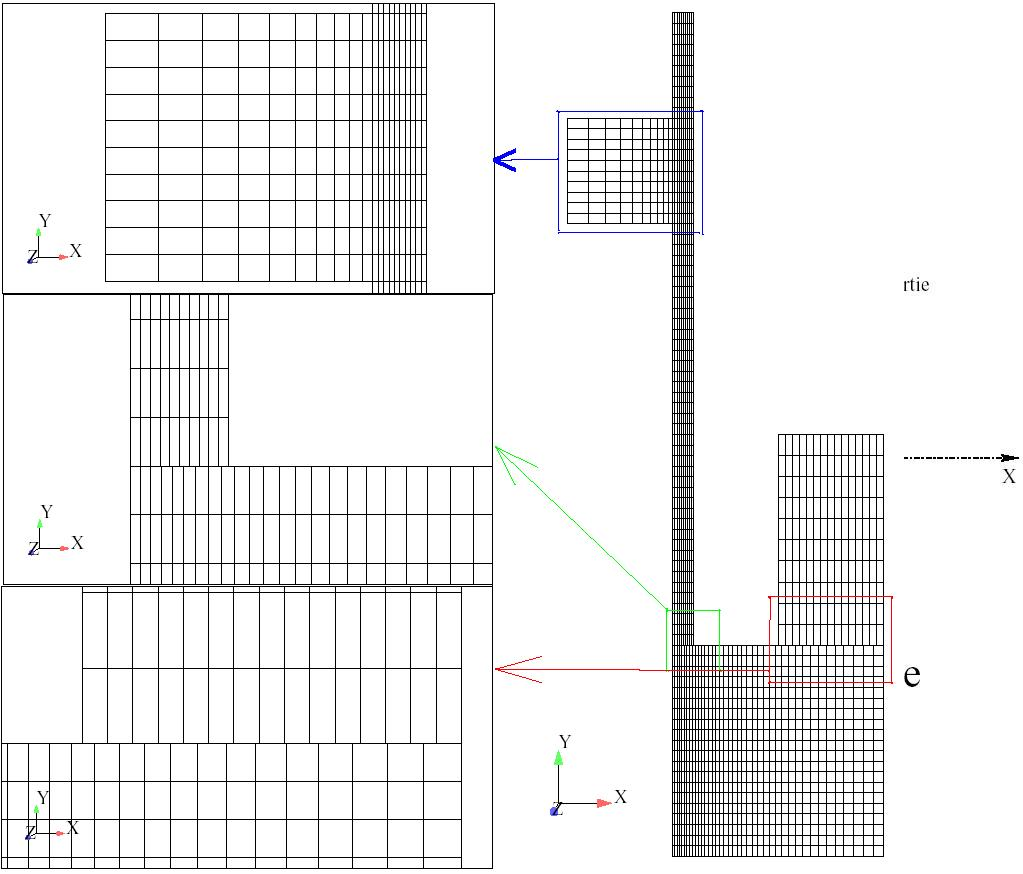
\includegraphics[width=8.65cm,height=7.4cm]{\repgraphics/fig05.jpg} 
\caption{View of the full domain mesh with zoom on the pasting regions}
\label{figante22}
\end{center}
\end{figure}

{\bfseries Type}: block structured mesh

{\bfseries Coordinates system}: cartesian, origin on the edge of the main
pipe at the outlet level, on the nozzle side (figure \ref{figante22})

{\bfseries Mesh generator used}: SIMAIL and mesh pasting with the Preprocessor
of \CS\ (in order to deal with hanging nodes)

{\bfseries Color definition}: see figure \ref{figante23} 

\begin{figure}[h!]
\begin{center}
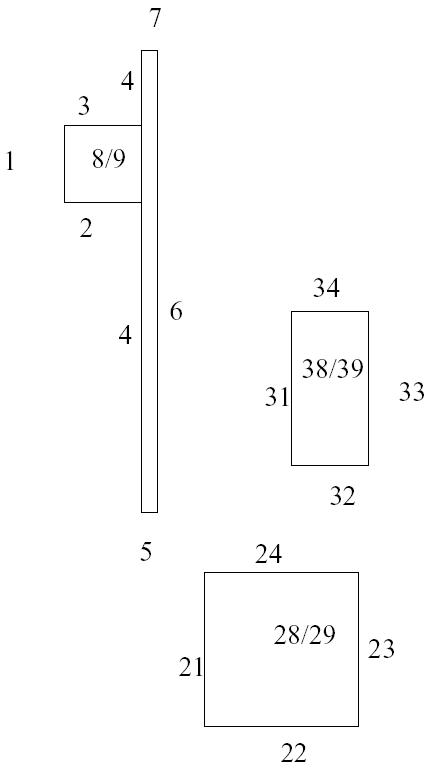
\includegraphics[width=3.6cm,height=6.4cm]{\repgraphics/fig06.jpg} 
\caption{Colors of the boundary faces}
\label{figante23}
\end{center}
\end{figure}


	\subsection{Summary of the different calculations}
%---------------------------------------------------------

Three cases will be studied with this geometry. The following table gives a
summary of their different characteristics.
\begin{center}
\begin{tabular}{|c|c|}
\hline
CASE & characteristics \\
\hline
CASE 2 & unsteady flow, additionnal passive scalar, output management \\
\hline
CASE 3 & same as case 2 with time dependent boundary conditions, \\ 
 &       fluid density depending on the temperature and calculation restart\\
\hline
CASE 4 & same as case 3 with head loss, parallelism and spatial average \\
\hline
\end{tabular}
\end{center}


%--------------------------------------------------------------------------------------
\section{CASE 2: Passive scalar with various boundary conditions and output management}
%--------------------------------------------------------------------------------------

	\subsection{Calculation options}
%-----------------------------------------

Some options are similar to case 1:
\begin{itemize}
\renewcommand{\labelitemi}{$\rightarrow$}
	\item Turbulence model: $k-\epsilon$
	\item Scalar(s): 1 - temperature
	\item Physical properties: uniform and constant
\end{itemize}

The new options are: 
\begin{itemize}
\renewcommand{\labelitemi}{$\rightarrow$}
	\item Flow type: unsteady flow
	\item Time step: uniform and constant
	\item Scalar(s): 2 - passive scalar\footnote{could correspond to a tracer
concentration for instance}
	\item Management of monitoring points
\end{itemize}


	\subsection{Initial and boundary conditions}
%---------------------------------------------------

\begin{itemize}
\renewcommand{\labelitemi}{$\rightarrow$}
	\item Initialization: 20\degresC\ for temperature (default value) \\
	\hspace*{2.1cm}        10 for the passive scalar
\end{itemize}


The boundary conditions are defined in the user interface and depend on the
boundary zone.

\begin{itemize}
	\item {\bfseries Flow inlet}: Dirichlet condition, an inlet velocity of
$1\ m.s^{-1}$, an inlet temperature of 300\degresC\ and an inlet value of 200
for the passive scalar are imposed
	\item {\bfseries Outlet}: default value
	\item {\bfseries Walls}: velocity, pressure and thermal scalar: default value \\
	            \hspace*{1.25cm} passive scalar: different conditions
depending on the color and geometric parameters
\end{itemize}

In order to test the ability to specify boundary condition regions in the
Graphical Interface, various conditions will be imposed for the passive scalar,
as specified in the following table:

\begin{center}
\begin{tabular}{|c|c|c|}
\hline
Wall & Nature & Value \\
\hline 
wall\_1 & Dirichlet  & 0 \\ 
\hline 
wall\_2 & Dirichlet  & 5 \\ 
\hline 
wall\_3 & Dirichlet  & 0 \\ 
\hline 
wall\_4 & Dirichlet  & 25 \\ 
\hline 
wall\_5 & Dirichlet  & 320 \\ 
\hline 
wall\_6 & Dirichlet  & 40 \\ 
\hline
\end{tabular} 
\end{center}

The ``wall\_1'' to ``wall\_6'' regions are defined as follows, through color
references and geometric localization:
\begin{center}
\begin{tabular}{c|c}
Label & Color and geometric parameters \\
\hline
wall\_1 & 24 and $0.1\leqslant X$ and $X\leqslant 0.5$ \\
wall\_2 & 2 or 3 \\
wall\_3 & 4 or 7 or 21 or 22 or 23 \\
wall\_4 & 6 and $Y>1$ \\
wall\_5 & 6 and $Y\leqslant1$ \\
wall\_6 & 31 or 33 \\
\end{tabular}
\end{center}

Figure \ref{figante23} shows the colors used for boundary conditions and 
table \ref{tabante21} defines the correspondance between the colors and  
the type of boundary condition to use.

\begin{table}[htp]
\begin{center}
\begin{tabular}{|c|c|} 
\hline
Colors & Conditions \\
\hline
1 & Inlet \\
\hline
34 & Outlet \\
\hline
2 3 4 6 7 21 22 23 24 31 33 & Wall \\
\hline
8 9 28 29 38 39 & Symmetry \\
\hline
\end{tabular}
\caption{Boundary faces colors and associated references}
\label{tabante21}
\end{center}
\end{table}


	\subsection{Parameters and User routines}
%------------------------------------------------

All parameters necessary to this study can be defined through the Graphical
Interface without using any user Fortran files.

\begin{center}
\begin{tabular}{|l|c|}
\hline
\multicolumn{2}{|c|}{Calculation control parameters} \\
\hline
Number of iterations & $300$ \\
\hline
Reference time step & $0.05$ \\
\hline
Output period for post-processing files& $2$ \\
\hline
\end{tabular}\\
\end{center}

In order to paste the separate meshes into a single domain, colors 5, 24 and 32
will have to be pasted through the Graphical Interface.



	\subsection{Output management}
%-------------------------------------

In this case, different aspects of output management will be addressed.

By default in the Graphical Interface, all variables are set to appear in the
listing, the post-processing and the chronological records. This default choice
can be modified by the user.

In this case, the {\itshape Pressure}, the {\itshape Tubulent energy} and the
{\itshape Dissipation} will be removed from the listing file.

The {\itshape Courant number} (CFL) and {\itshape Fourier number} will be
removed from the 
post-processing results\footnote{this can be very useful to save some disk space
if some variables are of no interest, as post-processing files can be large}.

Eventually, probes will be defined for chronological records, folowing the data
given in figure \ref{figante25}. Then the {\itshape total pressure} will be
deactivated for all probes and the {\itshape Velocity U} will only be activated
on probes  1, 2, 6, 7 and 8.

\begin{figure}[htp]
\parbox{8cm}{%
\centerline{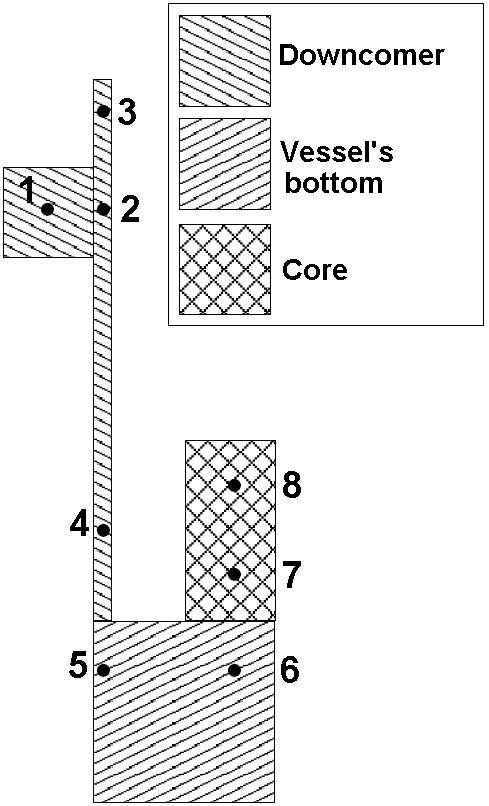
\includegraphics[width=4cm,height=6.8cm]{\repgraphics/fig07.jpg}}}
\parbox{7cm}{%
\begin{center}
\begin{tabular}{|c|c|c|c|}
\hline
Points & X(m) & Y(m) & Z(m)\\
\hline
1 & -0.25 & 2.25 & 0 \\
\hline
2 & 0.05 & 2.25 & 0 \\
\hline
3 & 0.05 & 2.75 & 0 \\
\hline
4 & 0.05 & 0.5 & 0 \\
\hline
5 & 0.05 & -0.25 & 0 \\
\hline
6 & 0.75 & -0.25 & 0 \\
\hline
7 & 0.75 & 0.25 & 0 \\
\hline
8 & 0.75 & 0.75 & 0 \\
\hline
\end{tabular}
\end{center}
}
\caption{Position and coordinates of probes in the full domain}
\label{figante25}
\end{figure}

In addition the domain boundary will be post-processed. This allows to check the
boundary conditions, and especially that of the passive scalar. 


	\subsection{Results}
%---------------------------

Figure \ref{fige1_e2} shows the boundary domain colored by the passive
scalar boundary conditions. The different regions of boundary
conditions defined earlier can be checked. 

\begin{figure}[h!]
\begin{center}
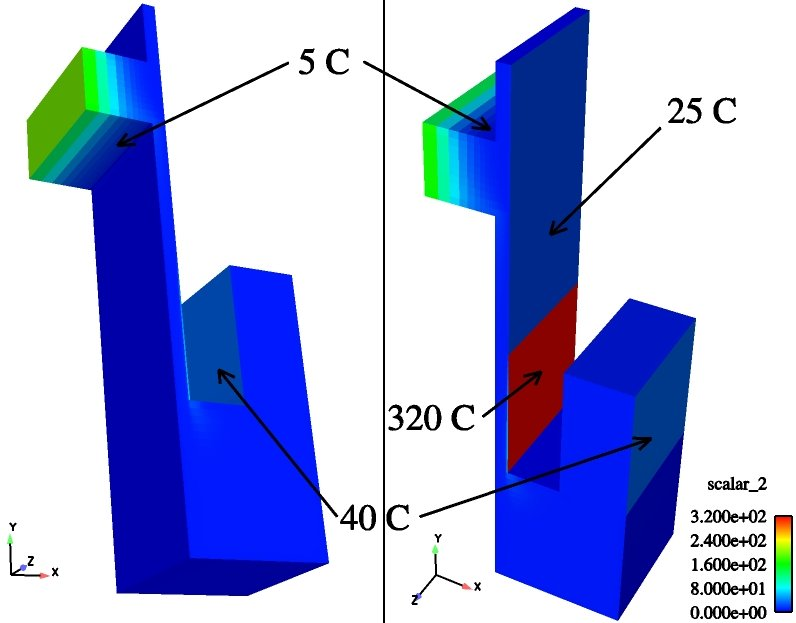
\includegraphics[width=14cm,height=11cm]{\repgraphics/c2_p7.jpg} 
\caption{View of the boundary domain colored by the scalar\_2 variable - Case 2}
\label{fige1_e2}
\end{center}
\end{figure}

Figure \ref{fige2_e2} presents results obtained at different times of the
calculation. They were plotted from the post-processing files, with EnSight.

\begin{figure}
\begin{center}
\begin{tabular}{cc}
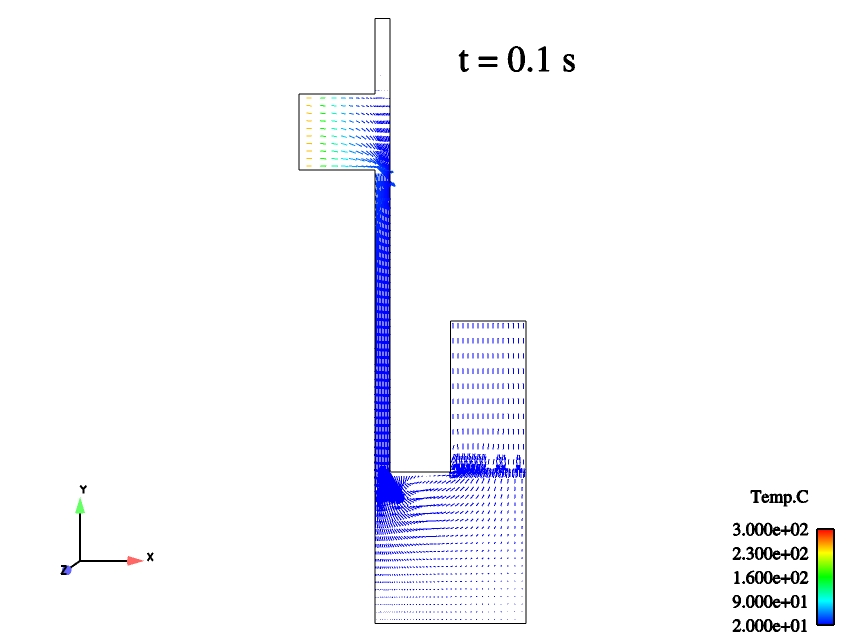
\includegraphics[width=6cm,height=6cm]{\repgraphics/c2_p1.jpg} & 
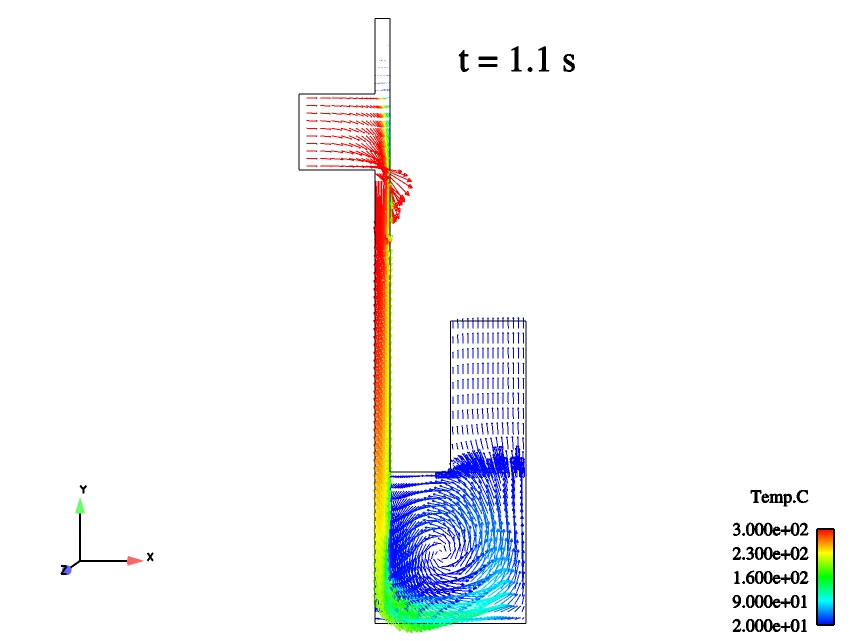
\includegraphics[width=6cm,height=6cm]{\repgraphics/c2_p2.jpg} \\
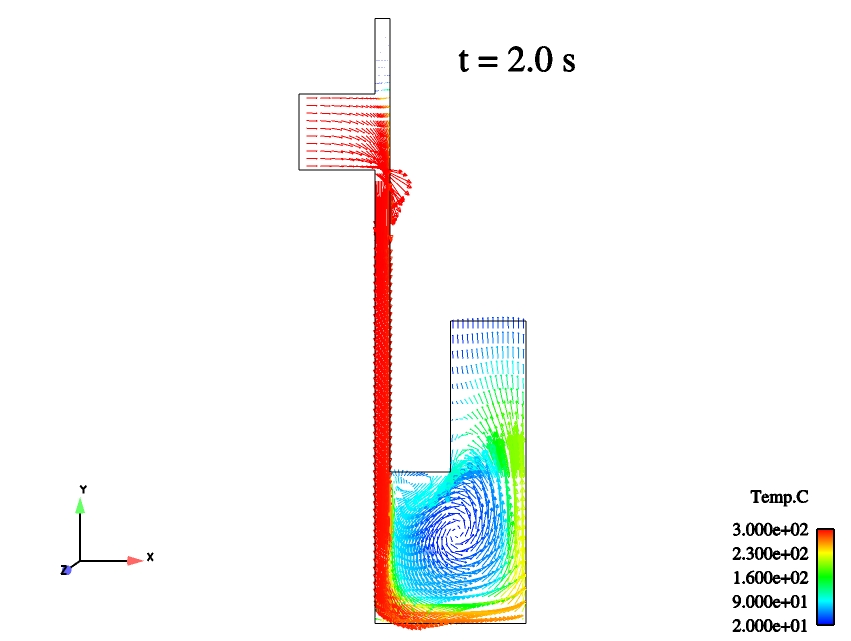
\includegraphics[width=6cm,height=6cm]{\repgraphics/c2_p3.jpg} & 
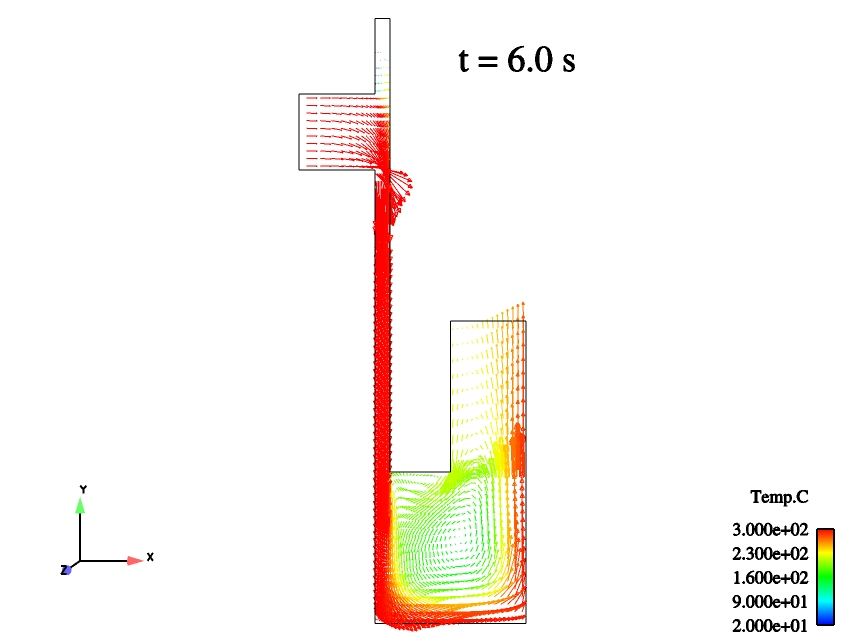
\includegraphics[width=6cm,height=6cm]{\repgraphics/c2_p4.jpg} \\
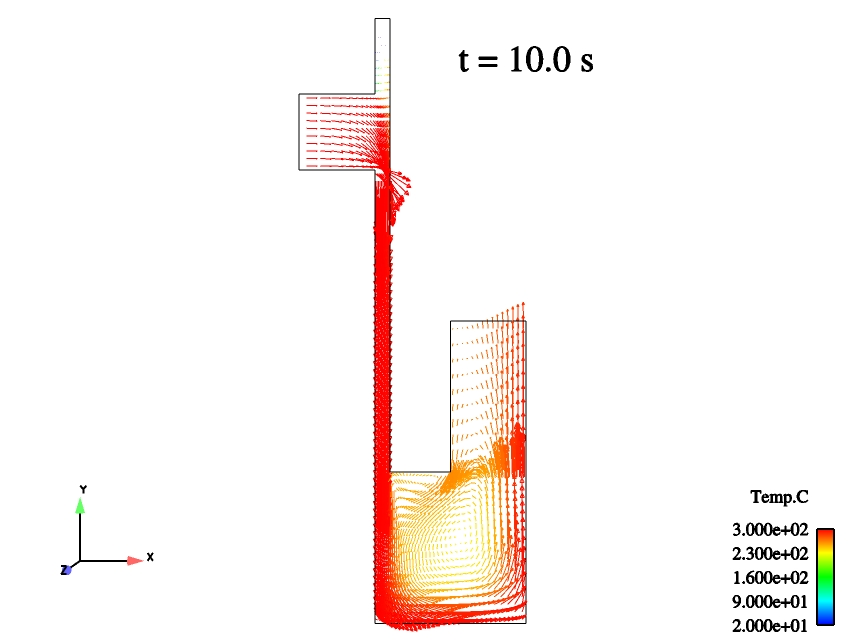
\includegraphics[width=6cm,height=6cm]{\repgraphics/c2_p5.jpg} & 
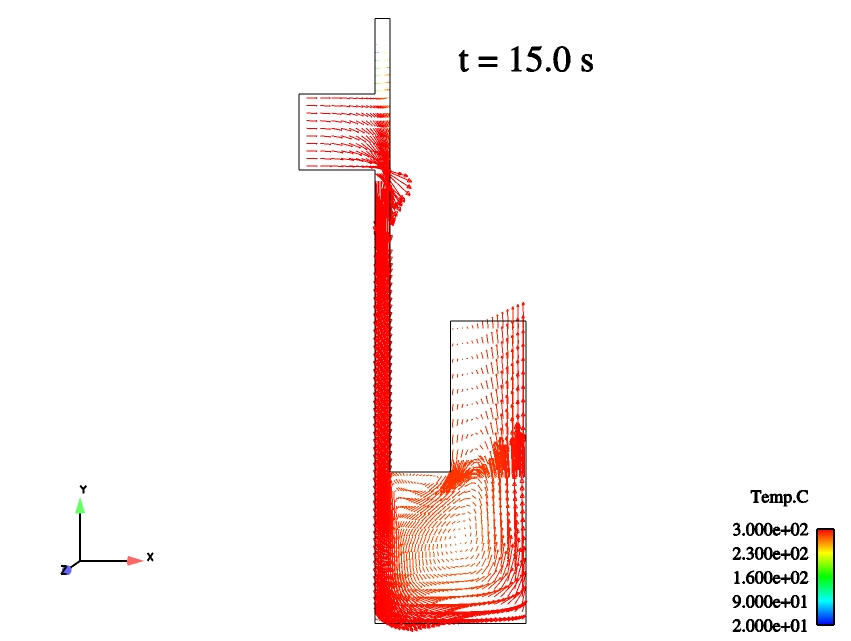
\includegraphics[width=6cm,height=6cm]{\repgraphics/c2_p6.jpg} \\
\end{tabular}
\caption{Water velocity field colored by temperature at different time steps - Case 2}
\label{fige2_e2}
\end{center}
\end{figure}
